% % % % % % % % % % % % % % % % % % % % % % % % % % % % % % % % % % % % % % % % 
% Formelsammlung von LaTeX4EI									
%
% @encode: 	UTF-8, tabwidth = 4, newline = LF
% @author:	Emanuel Regnath
% @date:		
%
% % % % % % % % % % % % % % % % % % % % % % % % % % % % % % % % % % % % % % % % 

%---------------------------------------%
%			Regelungssysteme			%
%~~~~~~~~~~~~~~~~~~~~~~~~~~~~~~~~~~~~~~~%

% Document Class ===============================================================
\documentclass[fs, footer]{latex4ei}

% DOCUMENT_BEGIN ===============================================================
\begin{document}

% Split in 4 Columns ===========================================================
\begin{multicols*}{4}

% TITLE ========================================================================
\fstitle{Regelungssysteme}

% SECTION ======================================================================
%\section*{Allgemeines} % (fold)
% ==============================================================================
%\label{sec:allgemeines}
%	\symbolbox{
%		\begin{tabular}{rl}
%			$a_{\ir soll}$ & Sollwert \\
%			$a_{\ir ist}$ & Istwert \\
%			$a_{\ir d}$ & Abstandsfehler, Regelfehler
%		\end{tabular}
%	}

%\sectionbox{
%	\emph{Manuelle Steuerung}
%	Istwert wird nicht zum Ausgleich des Abstandsfehlers herangezogen

%	\emph{Manuelle Regelung} 
%	$a_{\ir d}$ wird laufend erfasst und zur Korrektur herangezogen.
%}
% section allgemeines (end)

% SECTION ====================================================================================
\section{Der Regelkreis}
% ============================================================================================
\sectionbox{
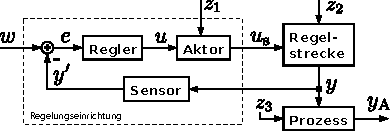
\includegraphics{./img/Regelkreis.pdf}

\tablebox{
	\begin{tabular*}{\columnwidth}{@{\extracolsep\fill}lll@{}} \ctrule
		Regelfehler & $e = w-y$ & Differenz zwischen „Soll“ und „Ist“\\
		Stellgröße & $u_{\ir S}$ & Eingang der Regelgröße\\ 
		Führungsgröße & $w$ & Sollverlauf, Vorgabe\\
		Aufgabengröße & $y_A$ & Die zu beinflussende Größe\\
		Regelgröße & $y$ & Die vom Sensor erfasste Größe\\
		Störgrößen & $z_i$ & Nicht beeinflussbare Störungen\\ \cbrule
	\end{tabular*} }
}

Zustand: Ausgang eines Integrators\\
\section{Modellbildung, Linearisierung, lin. Systeme}
\sectionbox{
	\subsection{Zustandsbeschreibung linearer Systeme}
	
	
	mit $r$ Erregungen, $n$ Zustandsgrößen und $k$ Ausgängen.\\
	Die Zustandsgrößen $\vec x$ müssen einen stetigen Verlauf haben!\\
	
	\tablebox{
		\begin{tabular*}{\columnwidth}{@{\extracolsep\fill}ll@{}} \ctrule
			Allgemeine Zustandsgleichung: & $\bs{ \dot {\vec x}}(t) = \ma A \vec x(t) + \ma B \vec v(t) $\\
			Allgemeine Ausgangsgleichung: & $\vec y(t) = \ma C \vec x(t) + \ma D \vec v(t)$ \\ \cmrule
			Zustandsvariable & $\vec x(t) \in \mathbb R^n$ \\
			Ausgangsvariable & $\vec y(t) \in \mathbb R^k$ \\
			Erregungsvektor & $\vec v \in \mathbb R^r$ \\
			Systemmatrix & $\ma A\in \mathbb R^{n \times n}$ \\
			Einkopplungsmatrix & $\ma B \in \mathbb R^{n \times r}$ \\
			Auskopplungsmatrix & $\ma C \in \mathbb R^{k \times n}$ \\
			Durchgangsmatrix & $\ma D \in \mathbb R^{k \times r}$ \\
			\cbrule
		\end{tabular*}
	}
	
	Falls $\ma A, \ma B, \ma C$ oder $\ma D$ zeitvariabel sind handelt es sich um ein LTV-System, falls nicht um ein LTI-System.
}
\sectionbox{

	\subsection{Linearisierung}
	Gegegeben (nicht linear): \quad $\vec{\dot x} = \vec f(\vec x, \vec u)$ \qquad \quad $\vec y = \vec g(\vec x, \vec u)$\\ 
	\subsubsection{um eine allg. Referenzlösung}

	-- todo --
	
	\subsubsection{um eine Ruhelaage}
	\begin{tabular}{ll}
	$\Delta \vec{\dot x} = \ma A \Delta \vec x + \ma B\Delta \vec u$ &  $\Delta \vec y = \ma C \Delta \vec x + \ma D\Delta \vec u$\\
	$\ma A = \left. \frac{\partial f_i}{\partial x_j} \right|_{(\vec x^*,\vec u^*)}$ & $\ma C = \left. \frac{\partial g_i}{\partial x_j} \right|_{(\vec x^*,\vec u^*)}$\\ 
	$\ma B = \left. \frac{\partial f_i}{\partial u_j} \right|_{(\vec x^*,\vec u^*)}$ & $\ma D = \left. \frac{\partial g_i}{\partial u_j} \right|_{(\vec x^*,\vec u^*)}$\\
	\end{tabular}
	

}



% ==============================================================================================
\section{Darstellung von LTI-SISO Systemen}
% ==============================================================================================

\sectionbox{	
	\subsection{Differentialgleichungen (DGL)}
	Gleichung mit Funktion $y$ und deren $n$-ten Ableitungen $y',y'',...$\\
	Allgemeine DGL $n$-ter Ordnung:\\ 
	$\displaystyle a_n y^{(n)} + ... + a_1 y' + a_0 y = b_m x^{(m)} + ... + b_1 x' + b_0 x$\\
	Gesucht ist eine Funktion $y$ und keine Zahl! In der Praxis werden DGLs numerisch für diskrete Werte gelöst.\\ 
	
	
	\subsubsection{DGL-Systeme}
	Jede DGL lässt sich reduzieren auf ein DGL-System 1. Ordnung:\\
	1. Substituiere $x_i := y^{(i-1)}$ und drücke $\dot x_i$ durch $x_1,...,x_n$ aus.\\
	$\Ra$ \boxed{ \dot{\vec x}(t) = \ma A \vec x(t) + \vec s(t) } \quad mit $\vec x_{\ir ges} = \vec x_{\ir hom} + \vec x_{\ir part}$\\
	Hom. Lösung: 1. Bestimme EW $\lambda_i$ und Basis aus EV $\vec b_i$ von $\ma A$\\
	2. $\vec x_{\ir hom} = \vec c \cdot e^{(x-x_0)\ma A} = \sum\limits_{i = 0}^n c_i \cdot e^{\lambda_i x} \cdot \vec b_i$\\
	3. Bestimmung der Konstanten durch einsetzen der Anfangsbedingungen!\	
}


\sectionbox{
	\subsection{Die Übertragungsfunktion}
	Beschreibt das System vollständig. Wird im Laplacebereich angegeben.\\ 
	Übertragungsfunktion einer lin. DGL $n$-ter Ordnung in Polynomform:\\
	\emphbox{ $\displaystyle G(s) = \frac{Y(s)}{U(s)} = \frac{\beta_k s^k + \ldots + \beta_1 s + \beta_0}{\alpha_r s^n + \ldots + \alpha_1 s + \alpha _0} = \frac{Z(s)}{N(s)}$ }
	($n =$ Ordnung der DGL $=$ Anzahl der Pole)\\
	\\
	Übertragungsfunktion der Zustandsbeschreibung:\\
	$\ma G (s) = \eset{\ma C (s \ma E - \ma A)^{-1} \ma B + \ma D}$\\
	für $q = r = 1$ (SISO-System):\\
	$G(s) = \eset{ \vec c^{T} (s \ma E - \ma A)^{-1} \vec b + d}$\\
	\\
	Linearfaktorenform: $G(s) = \frac{\beta_m}{\alpha_n} \frac{\prod (s-z_j)}{\prod (s-p_i)}$\\
	Zeitkonstantenform: $G(s) = \frac{\beta_0}{\alpha_0} \frac{\prod (1+T_v s)}{\prod (1+T s)}$\\
	Partialbruchform: $G(s) = A_0 \sum \frac{A_j}{s-p_j} = A_0 + G^+(s)$\\
	%$H(\cx s) := \frac{Y(\cx s)}{X(\cx s)} = \frac{\sum b_k s^k}{\sum a_i s^i}= k \frac{\prod (s-z_k)}{\prod (s-p_i)}$ \qquad $k = \frac{b_m}{a_n}$\\
	
	\subsubsection{Wichtige spezielle Übertragungsfunktionen (Frequenzantw.)}
	\begin{tabular}{@{}ll|ll}
		$u(t)$ & $U(s)$ & Zeitantwort & Frequenzantwort\\ \mrule
		$\delta(t)$ & $1$ & Impulsantw. $g(t)$ & Gewichtsfkt. $G(s)$\\
		$\sigma(t)$ & $\frac{1}{s}$ & Sprungantw. $h(t)$ & Übergangsfkt $H(s)$\\ 
		$t \cdot \sigma(t)$ & $\frac{1}{s^2}$ & Anstiegsantw. & Rampenantwort\\
		%$e^{\i \omega}$ & & Frequenzgang $H(\i \omega)$\\
	\end{tabular}\\
	
	
	Übertragungsfunktion des Reglers $G_{\ir R}(s)$\\
	Übertragungsfunktion des Stellers/Strecke $G_{\ir S}(s)$\\
	Übertragungsfunktion der Rückführung $G_{\ir r}(s)$\\
	Übertragungsfunktion des offenen Regelkreises $G_0(s) = G_{\ir R}(s) G_{\ir S}(s)$\\
	

	\subsubsection{Frequenzgang}
	Der FG ist die Systemantwort bei harmonischer Erregung $u(t) = e^{\i \omega t}$\\
	Nach dem Einschwingen (wird ignoriert) ist die Systemantwort ebenfalls harmonisch, allerdings mit anderer Amplitude und Phase.\\
	Frequenzgang: $G(\i \omega) = G(s)|_{s = 0 + \i \omega, \omega > 0} = A(\omega) e^{\i \varphi(\omega)}$
}


\sectionbox{
	\subsubsection{Zustandsraummodell}
	DGL $n$-ter Ordnung:\\ $a_n y^{(n)} + ... + a_1 y' + a_0 y = b_m x^{(m)} + ... + b_1 x' + b_0 x$\\
	Lässt sich immer reduzieren auf ein DGL-System 1. Ordnung:\\
	$\vec{\dot x} = \mat{0 & 1 & 0 & \ldots & 0 \\ 0 & 0 & 1 & \ldots & 0 \\ \ldots & \ldots & \ldots & \ldots & \ldots \\ 0 & 0 & 0 & \ldots & 1 \\ -a_0 & -a_1 & -a_2 & \ldots & -a_{n-1} }$ \\ \\
	
\emph{Normalformen} \\ \\
	\emph{Kanonische Normalform} \\
		zur Entkopplung des Systems bzw. der zugehörigen DGLs.
		
		Wähle $\ma T$ so das $\ma T^{-1} \ma A \ma T$ eine Diagonalmatrix ist:
		
		$\ma T^{-1} \ma A \ma T = \diag ( \lambda_i)$
		
		$\dot{\vec{x_k}} = \diag (\lambda_i) \vec x_k + \vec b_k u$
		
		$y = \vec{c_{k}^{T}} \vec{ x_{k}} + d u$ \\
		
		% ??? $G(s) = \sum \frac{A_k}{s - p_k}$
	\emph{Regelungsnormalform:} \\
		nur die letzte Zustandsvariable $x_{Rn}$ wird direkt durch den Eingang beeinflusst
		
		Steuerbarkeitsmatrix: $\ma S_S = \mat{\vec b & \ma A \vec b & \ma A^2 \vec b & \ldots & \ma A^{n-1} \vec b}$
		
		! RNF existiert nur falls $\ma S_S$ regulär ist $\ra $ System ist vollst. steuerbar
		
		Transformationsmatrix $\ma T_R = \mat{ \vec s_R^T \\ \vec s_R^T \ma A \\ \vec s_R^T \ma A^2 \\ \vdots \\ \vec s_R^T \ma A^{n-1}}^{-1}	$	
		
	\emph{Beobachtungsnormalform:} \\ 
		$\dot{\vec x }_B = \ma A_B \vec x_B + \vec b_B u$  \quad $\vec x_B (t_0) = \vec x_{B0}$
		
		$y = \vec c_B^T \vec x_B + d u$
		
		Beobachtbarkeitsmatrix $\ma S_B = \mat{ \vec c^T \\ \vec c^T \ma A \\ \vec c^T \ma A^2 \\ \vdots \\ \vec c^T \ma A^{n-1} }$
		
		Transformationsmatrix $\ma T_B = \mat{ \vec s_B & \ma A \vec s_B & \ldots & \ma A^{n-1} \vec s_b}$
		
		$\ma A_R = \ma A_B^T$ \quad $\vec b_R = \vec c_B$ \quad $\vec c_R = \vec b_B$
		
}
\sectionbox{
	\subsection{Schockschaltbildalgebra}
	\textbf{Serienschaltung:} $G(s) = \prod G_i(s)$\\
	\textbf{Parallelschaltung:} $G(s) = \sum G_i(s)$\\
	\textbf{Kreisstruktur:} $G(s) = \frac{G_{\ir Vor}(s)}{1 \mp G_{\ir Vor}(s) G_{\text{Rück}}(s)}$\\
}


\sectionbox{
	\subsection{Laplacetransformation}
	Anfangswertsatz: $y(t \ra \infty) = \lim\limits_{s \ra 0} [s G(s)U(s) ]$\\
	Endwertsatz: $y(t = 0^+)  = \lim\limits_{s \ra \infty} [s G(s)U(s) ]$\\
	Bleibender Regelfehler: $e(\infty) = u(\infty) - y(\infty)$\\
	
}



\section{Systembausteine}
\sectionbox{
	\subsection{P-System}
	$y(t) = K_{\ir P} u(t)$ \qquad $G(s) = K_{\ir P}$
	
	\subsection{I-System}
	$\dot y(t) = K_{\ir I} u(t)$ \qquad $G(s) = \frac{K_{\ir I}}{s}$

	\subsection{D-System}
	$y(t) = K_{\ir D} \dot u(t)$ \qquad $G(s) = K_{\ir D} s$

	\subsection{Totzeitsystem}
	$y(t) = K u(t-T_t)$ \qquad $G(s) = K e^{-s T_t}$
	
	\subsection{PT$_1$-Systeme}
	$T \dot y(t) + y(t) = K_{\ir P} u(t)$ \qquad $G(s) = \frac{K_{\ir P}}{1 +sT}$\\

	\subsection{PT$_2$-Systeme}
	$\ddot y(t) + 2D\omega_0 \dot y(t) + \omega_0^2 y = K_{\ir P} \omega_0^2 u(t)$\\
	$G(s) = K_{\ir P} \frac{\omega_0^2}{s^2 + 2D\omega_0 + \omega_0^2}$\\



	Einstellzeit $T_{\ir Ein}$ bis Signal im 5\% Bereich stabil.

% Tutoremail: artur.lohrer@gmx.de 
% Turium: 
% u* 1/(s^2+s a_0) + 



% Prüfung: Stab–Waagen Versuch Jacobimatrizen ausrechen!
% Passwort Moodle: rs1-2013


Übung:\\
1. Verschieben der Summationsstelle\\
2. Vertauschen/Zusammenfassen der Summationsstelle\\

$n$ Pole $\ne 0$ im Nenner: T$_n$ System\\
Allgemeine Polform: $p_{1/2} = \underbrace{-\omega_0 D}_{\sigma_e} \pm \i \underbrace{\omega_0 \sqrt{1 - D^2}}_{\omega_e}$\\ 
Dämpfung $D$ entscheidet ob System stabil: $D \le 0$: instabil
}




% SECTION ======================================================================
\section{Stabilität von Systemen}
% ==============================================================================
\sectionbox{
\subsection{Definitionen}
\textbf{stabil bzw. zustandsstabil:} $\norm{ \vec x_0 } < \varepsilon_1 \Ra \norm{ \vec x(t) } < \varepsilon_2$\\[1em]
\textbf{asymptotisch stabil:} zustandsstabil und $\lim\limits_{t \ra \infty} \norm{\vec x(t)} = 0$\\[1em]
\textbf{robust stabil:} bleibt auch bei Paramterabweichungen stabil.\\
Beispiel untersch. Systemmatrix: $\forall \ma A \in \eset{\ma A_{\min}; \ma A_{\max}}$ stabil
}

\sectionbox{
\subsubsection{Stabilitätsbedinung}
für LTI-Systeme

\emphbox{$\Re{\lambda_i (A)} < 0 \quad i = 1, \ldots, n$}
}

\sectionbox{
\subsection{Routh-Hurwitz-Kriterium}

	Gegeben:
	
	charakteristisches Polynom:
	$N(s) = b_n s^n + b_{n-1} s^{n-1} + \ldots + b_0$ \\
	
	Notwendige Bedingung:
	$b_i > 0 \quad \forall i \le n$ oder $b_i < 0 \quad \forall i \le n$\\

	
	Betrachte Koeffizienten $b_i$ des Nenners von $G(s)$\\
	\begin{tabular}{ll}
	$n = 1:$ & $b_1 > 0,\quad b_0 > 0$\\
	$n = 2:$ & $b_2 >0,\quad b_1 > 0,\quad b_0 > 0$\\	
	$n = 3:$ & $b_3 > 0,\quad b_2 > 0,\quad b_1 > 0,\quad b_0 > 0$\\	
			 & $b_2 b_1 - b_0 b_3 > 0$\\
	$n = 4:$ & $b_4 > 0,\quad b_3 > 0, \quad b_2 > 0, \quad b_1 > 0,\quad b_0 > 0$\\
			 & $b_3 b_2 b_1 - b_0 b_3^2 - b_1^2 b_4 > 0$\\
	\end{tabular}
	\\
	\emphbox{
	Ein System ist dann und nur dann stabil, wenn gilt:
	
	$b_n > 0$ und  alle $n$ Hurwitzdeterminanten $> 0$
	}
}
\sectionbox{
\subsection{Direkte Methode von Lyapunov}
	Betrachte nur Systemmatrix $\ma A$: \qquad \qquad \boxed{ \ma A^\top \ma P + \ma P \ma A = - \ma Q }\\
	1. Wähle $\ma Q = \ma E_n$ \quad 2. Berechne $\ma P$\\
	System asymptotisch stabil $\Longleftrightarrow$ $\ma P$ symm. und pos. definit\\		
}



\sectionbox{
\subsection{Eigenwerte und Polstellen}

%Systemmatrix $\ma A$: Alle EW $\lambda_i < 0$\\

	\subsubsection{Pole}
	Pole $p_i$ von $G(s)$: Alle $\Re{p_i} < 0$\\ 
	$G(s) = \sum \frac{k_i}{s-p_i}$ \qquad $\Ra \quad g(t) = \sum k_i e^{p_i t}$\\

	\subsubsection{Nyquist Kriterium}
	Betrachtet Ortskurve und Pole $p_{\ir links}, p_{\ir rechts}, p_{\ir auf}$ im Bezug auf die Imaginärachse.
	Das System ist stabil falls die OK nicht durch $-1 + 0\i$ verläuft und die Phasenänderung
	$W_{\ir soll} = \mathop{\Delta}\limits_{\omega = 0}^{\omega \ra \infty} \Phi = \pi p_{\ir rechts} + \frac{\pi}{2} p_{\ir auf}$


	\subsubsection{Dominanz im System}
	Vorraussetzung $T_{\max} > \tau_{\min}$\\
	Große Zeitkonstanten, Pole mit pos. Realteil (instabil),\\ 
}

\sectionbox{
\subsection{Zustandssteuerbarkeit und -beobachtbarkeit}
\textbf{zustandssteuerbar:} man kann $\vec x(t < \infty) = 0$ mit $\vec u(t)$ erreichen\\
\textbf{zustandsbeobachtbar:} man kann $\vec x_0$ aus $\vec y(t < \infty)$ bestimmen\\

}

\sectionbox{
\subsection{E/A (BIBO) Stabilität (äußere Stabilität)}

\emphbox{
\textbf{E/A Stabilität}

$\Re{p_i} < 0 \quad i = 1,2, \ldots n$
} \\

$\sum$ ist E/A-stabil, falls gilt:

\textbf{Definition:}
$\norm{ \vec u(t) } < \varepsilon_1 \Ra \norm{ \vec x(t) } < \varepsilon_2$ \\ 

\textbf{Pole der Übertragungsfunktion}:

$\Re{p_i} < 0 \quad i = 1,2, \ldots n$ \\ 

Stabilität Anhand von PN-Diagramm und Sprungantwort:\\
\setlength{\tabcolsep}{1mm}
\begin{tabular}{@{\extracolsep\fill}cccccc@{}} 
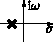
\includegraphics{./img/blocks/PN_1.pdf} & 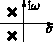
\includegraphics{./img/blocks/PN_2.pdf} & 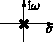
\includegraphics{./img/blocks/PN_3.pdf} & 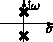
\includegraphics{./img/blocks/PN_4.pdf} & 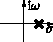
\includegraphics{./img/blocks/PN_5.pdf} & 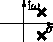
\includegraphics{./img/blocks/PN_6.pdf} \\
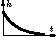
\includegraphics{./img/blocks/PN_1h.pdf} & 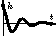
\includegraphics{./img/blocks/PN_2h.pdf} & 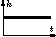
\includegraphics{./img/blocks/PN_3h.pdf} & 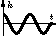
\includegraphics{./img/blocks/PN_4h.pdf} & 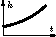
\includegraphics{./img/blocks/PN_5h.pdf} & 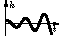
\includegraphics{./img/blocks/PN_6h.pdf} \\
stabil & stabil & stabil$^*$. & stabil$^*$ & instabil & instabil\\
\end{tabular}\\
$^*$: An der Stabilitätsgrenze.\\




\subsubsection*{Zusammenhang zwischen innerer und äußerer Stabilität}

Falls $\sum$ vollst. steuer- und beobachtbar, oder nur auf einer Untermenge steuer- und beobachtbar:

$\Ra$ asymptotisch stabil $\Leftrightarrow$ E/A-stabil
}


\sectionbox{
\subsection{Frequenzgangfunktion $G_0(\i \omega)$}
\pbox{4cm}{ 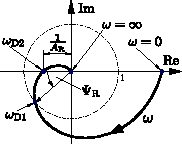
\includegraphics{./img/OK_G0.pdf} } \quad
\pbox{4cm}{ $A(\omega_{\ir D1}) = 1$ \qquad $\varphi(\omega_{\ir D2}) = -\pi$\\
$T_{\ir ein} \approx \frac{3}{\omega_{\ir D1}}$\\
\\
Stabilitätskriterien mit Totzeit:\\
geschl. RK ist E/A stabil falls:\\
Phasenrad $\Phi_{\ir R} > 0$\\
Amplitudenrand $A_{\ir R} > 1$\\
\\
$\Psi_{\ir R} \approx 30^\circ \Leftrightarrow $ gutes Störverhalten\\
$\Psi_{\ir R} \approx 60^\circ \Leftrightarrow $ gutes Folgeverhalten\\
}
}


% SECTION ======================================================================
\section{Grundlagen Reglerentwurf}
% ==============================================================================
Ziel: ideale Führung und ideal Störungsrobust $y(t) \stackrel{!}{=} 1 \cdot w(t) + \sum 0 z_i(t)$

$G_0(s) = G_{\ir R}(s) G_{\ir S}(s) G_{\ir r}(s)$



% Ende der Spalten
\end{multicols*}





% ###############################
\end{document}
% ###############################

\newpage

% Split in 2 Columns ===========================================================
\begin{multicols*}{2}


\begin{tabular*}{\columnwidth}{@{\extracolsep\fill}llll@{}} \ctrule
			& DGL & $G(s)$ & Sprungantwort $g(t)$\\
\textbf{P} & $y(t) = K_{\ir P} u(t)$ & $G(s) = K_{\ir P}$ & 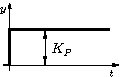
\includegraphics{./img/blocks/P_G.pdf}\\
\textbf{I} & $\dot y(t) = K_{\ir I} u(t)$ & $G(s) = \frac{K_{\ir I}}{s}$ \\
\textbf{D} & $y(t) = K_{\ir D} \dot u(t)$ & $G(s) = K_{\ir D} s$ \\
\textbf{T}$_t$ & \\


\textbf{PID} & \\
\textbf{PIDT}$_1$ & \\
\end{tabular*}



\subsection{Auswahl von Reglern}
% Siehe copy46ef79649f541 Seite 34
\begin{tabular}{ll|lllll}
 & Strecke & Regler \\
Typ & Beispiel & P & I & PI & PD & PID\\
P & Durchfluss & u & gg & & u & za \\
PT$_1$ & Druck & \\
PT$_n$ & Temperatur & \\
IT$_n$ & Füllstand & & i & gS & ggF & ggS\\
I$_2$ & Kurs & i & \\
\end{tabular}


\end{multicols*}

% Midterm: Anfangs und Endwertsatz wichtig!

% Dokumentende
% ======================================================================
\end{document}

% ToDos:

